\begin{figure}[htb]
\centering
\begin{tikzpicture}[scale = 10]
\tikzstyle{VertexStyle}=[shape = circle,	
								 minimum size = 1pt,
								 inner sep = 1.2pt,
                         draw]
\Vertex[x = 0.491999983787537, y = 0.856000006198883, L = \tiny {$x_1$}]{v0}
\Vertex[x = 0.586000025272369, y = 0.761999994516373, L = \tiny {$x_2$}]{v1}
\Vertex[x = 0.389999985694885, y = 0.758000001311302, L = \tiny {$x_5$}]{v2}
\Vertex[x = 0.420000016689301, y = 0.631999999284744, L = \tiny {$x_4$}]{v3}
\Vertex[x = 0.555999994277954, y = 0.629999965429306, L = \tiny {$x_3$}]{v4}
\Vertex[x = 0.811999976634979, y = 0.765999987721443, L = \tiny {$y$}]{v5}
\Edge[](v1)(v0)
\Edge[](v1)(v4)
\Edge[](v4)(v3)
\Edge[](v2)(v3)
\Edge[](v0)(v2)
\Edge[](v5)(v0)
\Edge[](v5)(v1)
\Edge[](v5)(v4)
\Edge[](v5)(v3)
\end{tikzpicture}
\caption{The graph $N_6$.}
\label{fig:N6}
\end{figure}
